\documentclass[a4paper,12pt]{article}
\usepackage[utf8]{inputenc}
\usepackage[german]{babel}
\usepackage{amsmath}
\usepackage{amssymb}
\usepackage{amsthm}
\usepackage{geometry}
\usepackage{graphicx}
\usepackage[hidelinks]{hyperref}
\usepackage{listings}
\usepackage{xcolor}
\usepackage{enumitem}
\usepackage{booktabs}
\usepackage{array}
\usepackage{caption}
\usepackage{subcaption}

\geometry{margin=2.5cm}

\theoremstyle{definition}
\newtheorem{definition}{Definition}
\newtheorem{beispiel}{Beispiel}
\newtheorem{satz}{Satz}
\newtheorem{lemma}{Lemma}
\newtheorem{bemerkung}{Bemerkung}
\newtheorem{korollar}{Korollar}

\setlist[itemize,1]{label=--}

% ---------- Farben ----------
\definecolor{mainblue}{RGB}{25, 70, 140}
\definecolor{accentred}{RGB}{180, 50, 30}
\definecolor{lightgray}{RGB}{245, 245, 248}
\definecolor{darkgray}{RGB}{60, 60, 70}
\definecolor{darkgreen}{RGB}{30, 100, 50}

\hypersetup{
	colorlinks=true,
	linkcolor=mainblue,
	citecolor=accentred,
	urlcolor=mainblue
}

\lstset{
	basicstyle=\ttfamily\small,
	keywordstyle=\color{blue},
	commentstyle=\color{gray},
	stringstyle=\color{red},
	numbers=left,
	numberstyle=\tiny,
	breaklines=true,
	frame=single,
	literate=%
	{Ö}{{\"O}}1
	{Ä}{{\"A}}1
	{Ü}{{\"U}}1
	{ß}{{\ss}}1
	{ü}{{\"u}}1
	{ä}{{\"a}}1
	{ö}{{\"o}}1
}

\title{\textbf{HIV-Infektion:}\\[0.4em]
\large Molekulare Mechanismen, Epidemiologie und\\
mathematische Modellierung der Infektionsdynamik}
\author{Stephan Epp\\
\small Universit\"at Bielefeld -- Fakult\"at f\"ur Informatik\\
\small \texttt{stephan.epp@uni-bielefeld.de}}
\date{Mai 2026}

\begin{document}

\maketitle

\begin{abstract}
Das humane Immundefizienz-Virus (HIV) hat seit seiner Entdeckung im Jahr 1983 mehr als 40 Millionen
Menschenleben gefordert und stellt eine der gravierendsten globalen Gesundheitskrisen der
Menschheitsgeschichte dar~\cite{bekker2023hiv}.
Diese Arbeit pr\"asentiert eine formale und mathematisch rigorose Analyse der HIV-Infektionsdynamik,
des Replikationszyklus sowie der epidemiologischen Ausbreitung.
Wir formulieren das Within-Host-Modell (Target-Cell-Limited-Modell nach Perelson et al.)
als System gew\"ohnlicher Differentialgleichungen und beweisen formal die Bedingungen
f\"ur virale Persistenz, Suppressionsgleichgewichte und Eliminationskriterien.
Dar\"uber hinaus analysieren wir ein erweitertes SI-Modell auf Bev\"olkerungsebene,
berechnen die Basisreproduktionszahl~$R_0$ und zeigen, dass antiretrovirale Therapie (ART)
mit hoher Abdeckung hinreichend ist, $R_0 < 1$ zu erreichen und damit epidemische Ausbreitung
zu verhindern. Alle Ergebnisse werden durch numerische Simulationen und Abbildungen illustriert.
\end{abstract}

\tableofcontents
\newpage

% =============================================================================
\section{Einf\"uhrung}
% =============================================================================

\subsection{Historischer \"Uberblick}

Die AIDS-Epidemie geh\"ort zu den folgenreichsten Infektionskrankheiten der modernen Geschichte.
Im Jahr 1981 wurden in den USA die ersten F\"alle einer r\"atselhaften Immunschw\"ache
beobachtet, die sp\"ater als \emph{Acquired Immunodeficiency Syndrome} (AIDS) bezeichnet wurde.
1983 isolierten Barr\'e-Sinoussi und Montagnier in Paris erstmals den verantwortlichen Erreger
-- das Humane Immundefizienz-Virus (HIV) --, wof\"ur sie 2008 den Nobelpreis f\"ur Medizin erhielten.

Seit Beginn der Epidemie hat das Virus mehr als \textbf{85 Millionen} Menschen infiziert und
\"uber \textbf{40 Millionen Todesfälle} verursacht~\cite{bekker2023hiv}. Ende 2023 lebten
weltweit rund 39,9 Millionen Menschen mit HIV. Trotz dieser enormen Last hat die Entwicklung
hochwirksamer antiretroviraler Therapien (ART) seit Mitte der 1990er-Jahre die Prognose der
Erkrankung fundamental ver\"andert: HIV-Infektion ist heute f\"ur Personen mit Zugang zu ART
eine chronisch behandelbare Erkrankung mit nahezu normaler Lebenserwartung.

\begin{figure}[h]
\centering
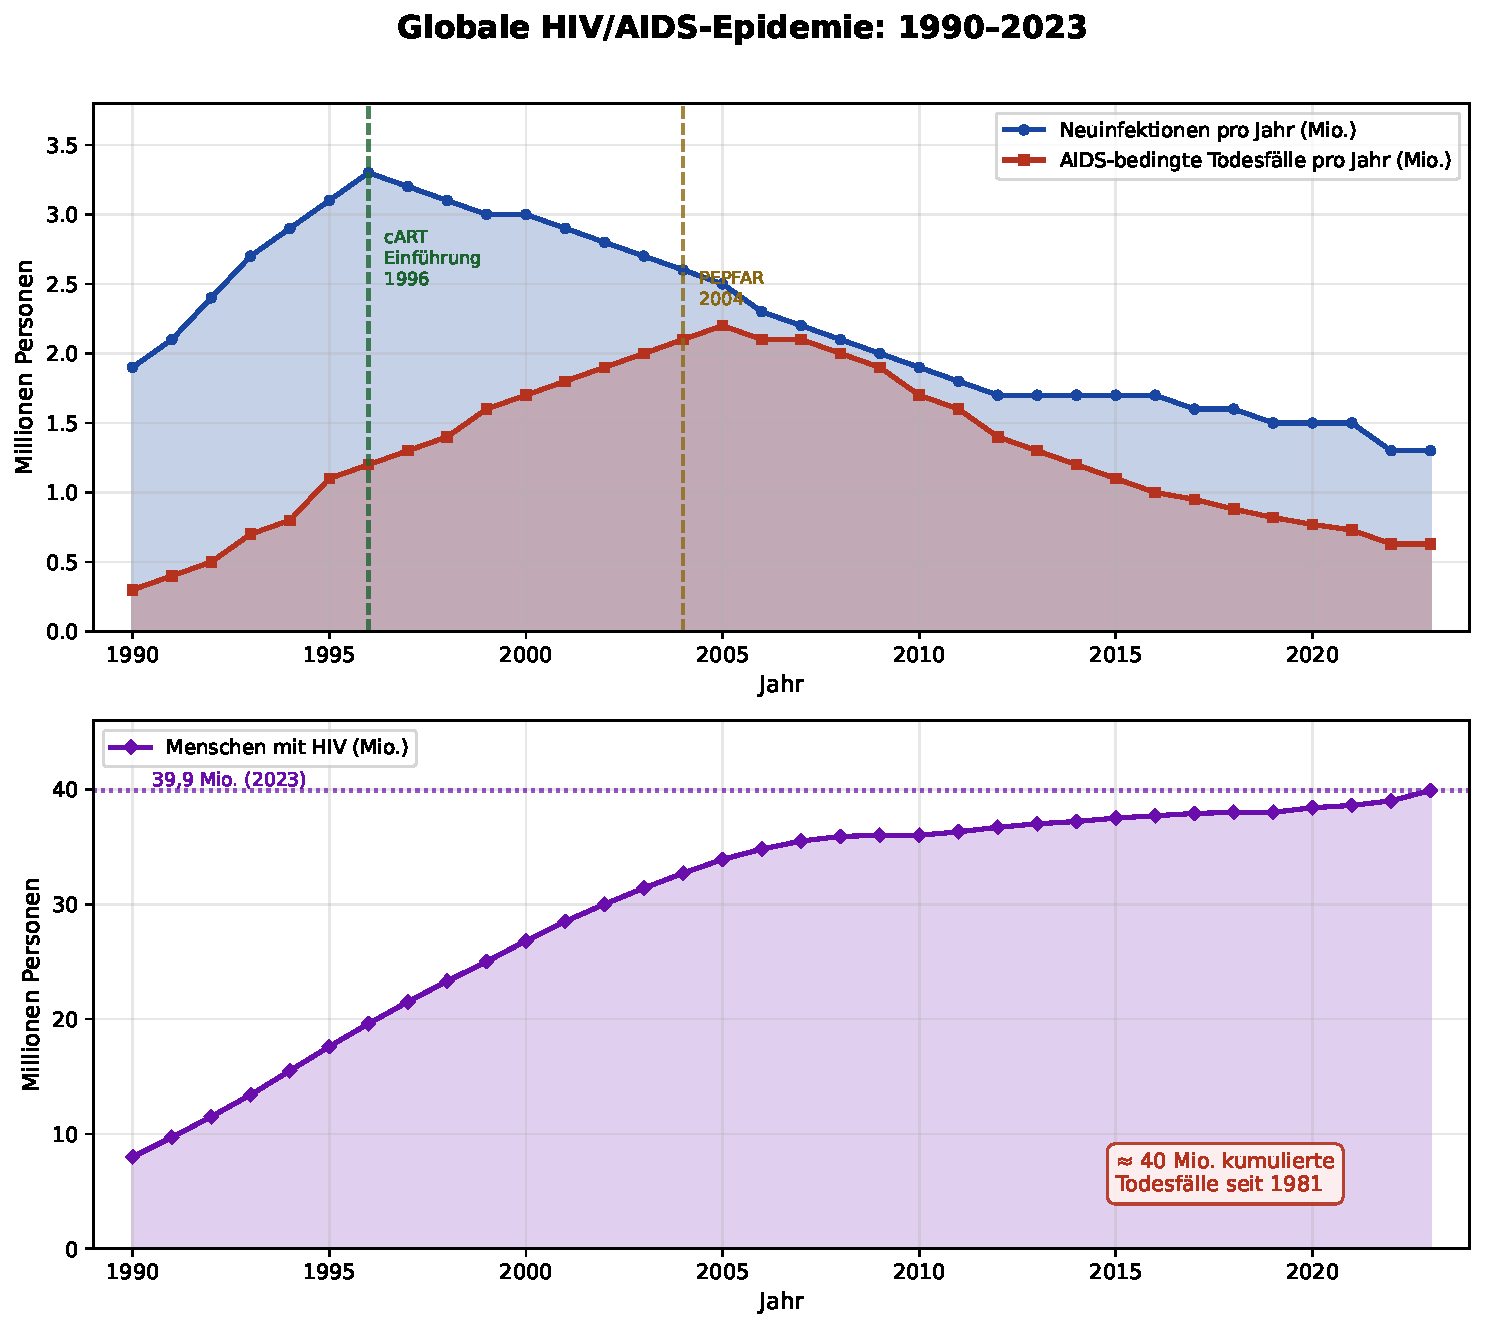
\includegraphics[width=0.92\textwidth]{plot1_epidemic.pdf}
\caption{Globale HIV/AIDS-Epidemiekurve 1990--2023. \textbf{Oben:} Neuinfektionen und
AIDS-bedingte Todesfälle pro Jahr. Die Einf\"uhrung der kombinierten antiretroviralen
Therapie (cART, 1996) und die US-amerikanische PEPFAR-Initiative (2004) markieren
kritische Wendepunkte. \textbf{Unten:} Gesamtzahl der Menschen mit HIV.
Daten: UNAIDS World AIDS Day Report 2023.}
\label{fig:epidemic}
\end{figure}

\subsection{Problemstellung}

Der Verlauf einer HIV-Infektion ohne Therapie lässt sich in drei Phasen unterteilen:

\begin{enumerate}
\item \textbf{Akute Phase} (Wochen 1--6): Rasche virale Replikation, hohe Viruslast,
      transiente Reduktion der CD4$^+$ T-Zellzahl, grippeähnliche Symptome.
\item \textbf{Chronische Phase} (Monate bis Jahre): Klinische Latenz, moderater Abfall der
      CD4$^+$ T-Zellen, niedrige bis moderate Viruslast.
\item \textbf{AIDS-Stadium} (nach Abfall des CD4-Wertes unter 200 Zellen/$\mu$L): Schwere
      Immundefizienz, opportunistische Infektionen, Tod innerhalb von 2--10 Jahren.
\end{enumerate}

\textbf{Zentrale biologische Fragen:}
\begin{itemize}
\item Wie infiziert HIV-1 Wirtszellen über CD4, CCR5 und CXCR4?
\item Welche mathematischen Gesetze beschreiben die Within-Host-Dynamik?
\item Unter welchen formalen Bedingungen ist virale Suppression durch ART erreichbar?
\item Wie lässt sich die epidemische Ausbreitung formal kontrollieren?
\end{itemize}

\subsection{Motivation}

Das formale Verständnis der HIV-Dynamik ist aus mehreren Gr\"unden essenziell:
Erstens erlaubt es die pr\"azise Vorhersage des Krankheitsverlaufs und die Optimierung
von Therapieregimen. Zweitens erm\"oglicht die mathematische Modellierung der
Epidemiologie die Planung wirksamer pr\"aventiver Interventionen.
Drittens ist die Quantifizierung der Basisreproduktionszahl $R_0$ fundamental
f\"ur das Verst\"andnis, unter welchen Bedingungen ART als \emph{Treatment as Prevention}
(TasP) eine Eliminierung der Epidemie erm\"oglicht.

% =============================================================================
\section{Grundlagen}
% =============================================================================

\subsection{Biologische Definitionen}

\begin{definition}[HIV-1-Virion]
Ein HIV-1-Virion ist ein sph\"arisches Retrovirus der Familie \emph{Retroviridae},
Gattung \emph{Lentivirus}, mit einem Durchmesser von ca.\ 120\,nm.
Das Genom besteht aus zwei identischen, positiv-orientierten ssRNA-Str\"angen
mit je $\approx 9{,}7$\,kb, enkodierend die Gene \texttt{gag}, \texttt{pol}, \texttt{env}
und sechs akzessorische Gene (\texttt{tat}, \texttt{rev}, \texttt{nef}, \texttt{vif},
\texttt{vpr}, \texttt{vpu}).
\end{definition}

\begin{definition}[Zielzelle]
Eine Zielzelle $T$ ist eine Wirtszelle, die den Oberfl\"achenrezeptor CD4 sowie
einen der Korezeptoren CCR5 oder CXCR4 exprimiert. Haupts\"achlich betroffen sind
CD4$^+$ T-Lymphozyten, Makrophagen und dendritische Zellen.
\end{definition}

\begin{definition}[Viruslast]
Die Viruslast $V(t) \in \mathbb{R}_{\geq 0}$ bezeichnet die Konzentration infekti\"oser
HIV-1-RNA-Kopien pro Milliliter Blutplasma zur Zeit $t$, gemessen in Kopien/mL.
Klinisch definierte Schwellenwerte:
\begin{align*}
V(t) &< 50 \quad \Rightarrow \quad \text{Virussuppression (``undetectable'')} \\
V(t) &> 1000 \quad \Rightarrow \quad \text{Therapieversagen (WHO-Definition)}
\end{align*}
\end{definition}

\begin{definition}[CD4-Zellzahl]
Die CD4-Zellzahl $T(t) \in \mathbb{R}_{\geq 0}$ bezeichnet die Konzentration nicht-infizierter
CD4$^+$ T-Lymphozyten pro Mikroliter Vollblut. Referenzwert gesunder Erwachsener:
$T_0 \approx 500$--$1600$ Zellen/$\mu$L. AIDS ist definiert durch $T(t) < 200$ Zellen/$\mu$L.
\end{definition}

\begin{definition}[Basisreproduktionszahl]
Die Basisreproduktionszahl $R_0 \in \mathbb{R}_{\geq 0}$ gibt an, wie viele Sekund\"arinfektionen
ein einzelnes Virus (oder eine infizierte Person) im vollst\"andig suszeptiblen System
im Durchschnitt erzeugt. Es gilt:
\[
R_0 > 1 \;\Leftrightarrow\; \text{Infektion breitet sich aus}, \qquad
R_0 < 1 \;\Leftrightarrow\; \text{Infektion stirbt aus}.
\]
\end{definition}

\subsection{HIV-Replikationszyklus}

Der Replikationszyklus von HIV-1 in einer Zielzelle verl\"auft in acht definierten Schritten:

\begin{enumerate}
\item \textbf{Adsorption}: Das Hüllprotein gp120 bindet an den CD4-Rezeptor.
      Diese Bindung induziert eine Konformations\"anderung.
\item \textbf{Korezeptorbindung}: Konformations-ge\"andertes gp120 bindet an CCR5
      (bei R5-trop-hem Virus) oder CXCR4 (bei X4-trophem Virus).
\item \textbf{Fusion}: Das Hüllprotein gp41 vermittelt die Fusion der viralen Hülle
      mit der Zellmembran; das Kapsid gelangt ins Zytoplasma.
\item \textbf{Reverse Transkription}: Die virale Reverse Transkriptase (RT) synthetisiert
      aus der ssRNA eine doppelsträngige DNA (dsDNA).
\item \textbf{Import}: Der Pr\"aintegrationskomplex (PIC) wird in den Kern importiert.
\item \textbf{Integration}: Die virale Integrase katalysiert die kovalente Integration
      der viralen DNA in das Wirtszellgenom (Provirus).
\item \textbf{Transkription und Translation}: Das Provirus wird durch zelluläre und virale
      Faktoren (Tat) transkribiert; virale Proteine werden synthetisiert.
\item \textbf{Reifung und Knospung}: Neue Virionen knospen aus der Zellmembran;
      die virale Protease spal-tet Gag- und Gag-Pol-Vorläufer zur Reifung.
\end{enumerate}

\subsection{Pharmakologische Angriffspunkte}

Jeder Schritt des Replikationszyklus ist ein potenzieller Angriffspunkt f\"ur ART:

\begin{center}
\begin{tabular}{lll}
\toprule
\textbf{Schritt} & \textbf{Wirkstoffklasse} & \textbf{Beispiel} \\
\midrule
Fusion           & Fusionsinhibitoren       & Enfuvirtid (T-20) \\
Korezeptorbindung & CCR5-Antagonisten       & Maraviroc \\
Reverse Transkription & NRTI, NNRTI        & Tenofovir, Efavirenz \\
Integration      & Integrase-Inhibitoren    & Dolutegravir \\
Reifung          & Protease-Inhibitoren     & Darunavir \\
Kapsidfunktion   & Kapsid-Inhibitoren       & Lenacapavir \\
\bottomrule
\end{tabular}
\end{center}

% =============================================================================
\section{Mathematische Modellierung der Within-Host-Dynamik}
% =============================================================================

\subsection{Das Target-Cell-Limited-Modell}

Das grundlegende mathematische Modell der HIV-Within-Host-Dynamik geht auf die Arbeiten
von Perelson et al.~(1993, 1996) zur\"uck. Es beschreibt die Wechselwirkung zwischen
nicht-infizierten Zielzellen $T$, infizierten Zellen $I$ und freien Viren $V$ als System
gew\"ohnlicher Differentialgleichungen (ODEs):

\begin{align}
\frac{dT}{dt} &= \lambda - d_T \cdot T - \beta \cdot T \cdot V \label{eq:dT} \\
\frac{dI}{dt} &= \beta \cdot T \cdot V - \delta \cdot I \label{eq:dI} \\
\frac{dV}{dt} &= p \cdot I - c \cdot V \label{eq:dV}
\end{align}

mit den Parametern:
\begin{center}
\begin{tabular}{lll}
\toprule
\textbf{Parameter} & \textbf{Bedeutung} & \textbf{Typischer Wert} \\
\midrule
$\lambda$  & Produktionsrate nicht-infizierter T-Zellen  & $10^4$ Zellen/mL/Tag \\
$d_T$      & Sterberate nicht-infizierter T-Zellen       & $0{,}01$ /Tag \\
$\beta$    & Infektionsrate                              & $2{,}4 \times 10^{-8}$ mL/(Kopie$\cdot$Tag) \\
$\delta$   & Sterberate infizierter Zellen               & $0{,}7$ /Tag \\
$p$        & Virale Produktionsrate pro infizierter Zelle& 300 Kopien/Zelle/Tag \\
$c$        & Virale Clearance-Rate                       & $3{,}0$ /Tag \\
\bottomrule
\end{tabular}
\end{center}

\subsection{Gleichgewichtspunkte und Stabilit\"atsanalyse}

\begin{definition}[Infektionsfreies Gleichgewicht]
Das infektionsfreie Gleichgewicht $E_0$ des Systems (\ref{eq:dT})--(\ref{eq:dV}) ist
\[
E_0 = \left(T_0^*, 0, 0\right) = \left(\frac{\lambda}{d_T}, 0, 0\right).
\]
\end{definition}

\begin{definition}[Endemisches Gleichgewicht]
Das endemische (infekti\"ose) Gleichgewicht $E^*$ ist definiert als
\[
E^* = (T^*, I^*, V^*),
\]
wobei alle Komponenten strikt positiv sind, d.\,h.\ $T^*, I^*, V^* > 0$.
\end{definition}

\begin{lemma}[Berechnung des endemischen Gleichgewichts]
\label{lem:eq_endemic}
Im endemischen Gleichgewicht $E^*$ gelten folgende Beziehungen:
\[
T^* = \frac{c \cdot \delta}{\beta \cdot p}, \qquad
I^* = \frac{\lambda}{{\delta}} - \frac{d_T \cdot c}{\beta \cdot p}, \qquad
V^* = \frac{p}{{c}} \cdot I^*.
\]
\end{lemma}

\begin{proof}
Im Gleichgewicht gilt $\frac{dT}{dt} = \frac{dI}{dt} = \frac{dV}{dt} = 0$.

\textbf{Aus Gleichung (\ref{eq:dV}):}
\[
p \cdot I^* = c \cdot V^* \quad\Rightarrow\quad V^* = \frac{p}{c} \cdot I^*.
\]

\textbf{Aus Gleichung (\ref{eq:dI}):}
\[
\beta \cdot T^* \cdot V^* = \delta \cdot I^* \quad\Rightarrow\quad
T^* = \frac{\delta \cdot I^*}{\beta \cdot V^*} = \frac{\delta \cdot I^*}{\beta \cdot \frac{p}{c} \cdot I^*}
     = \frac{\delta \cdot c}{\beta \cdot p}.
\]

\textbf{Aus Gleichung (\ref{eq:dT}):}
\[
\lambda = d_T \cdot T^* + \beta \cdot T^* \cdot V^*
        = T^* (d_T + \beta \cdot V^*)
        = T^* \left(d_T + \frac{\beta \cdot p}{c} \cdot I^*\right).
\]
Einsetzen von $T^* = \frac{c \delta}{\beta p}$:
\[
\lambda = \frac{c\delta}{\beta p} \cdot d_T + \delta \cdot I^*
\quad\Rightarrow\quad
I^* = \frac{\lambda}{\delta} - \frac{d_T \cdot c}{\beta \cdot p}.
\]
Das endemische Gleichgewicht existiert genau dann, wenn $I^* > 0$, also wenn
$\frac{\lambda}{\delta} > \frac{d_T \cdot c}{\beta \cdot p}$, was \"aquivalent zu $R_0 > 1$ ist
(vgl.\ Satz~\ref{satz:R0}).
\end{proof}

\begin{figure}[h]
\centering
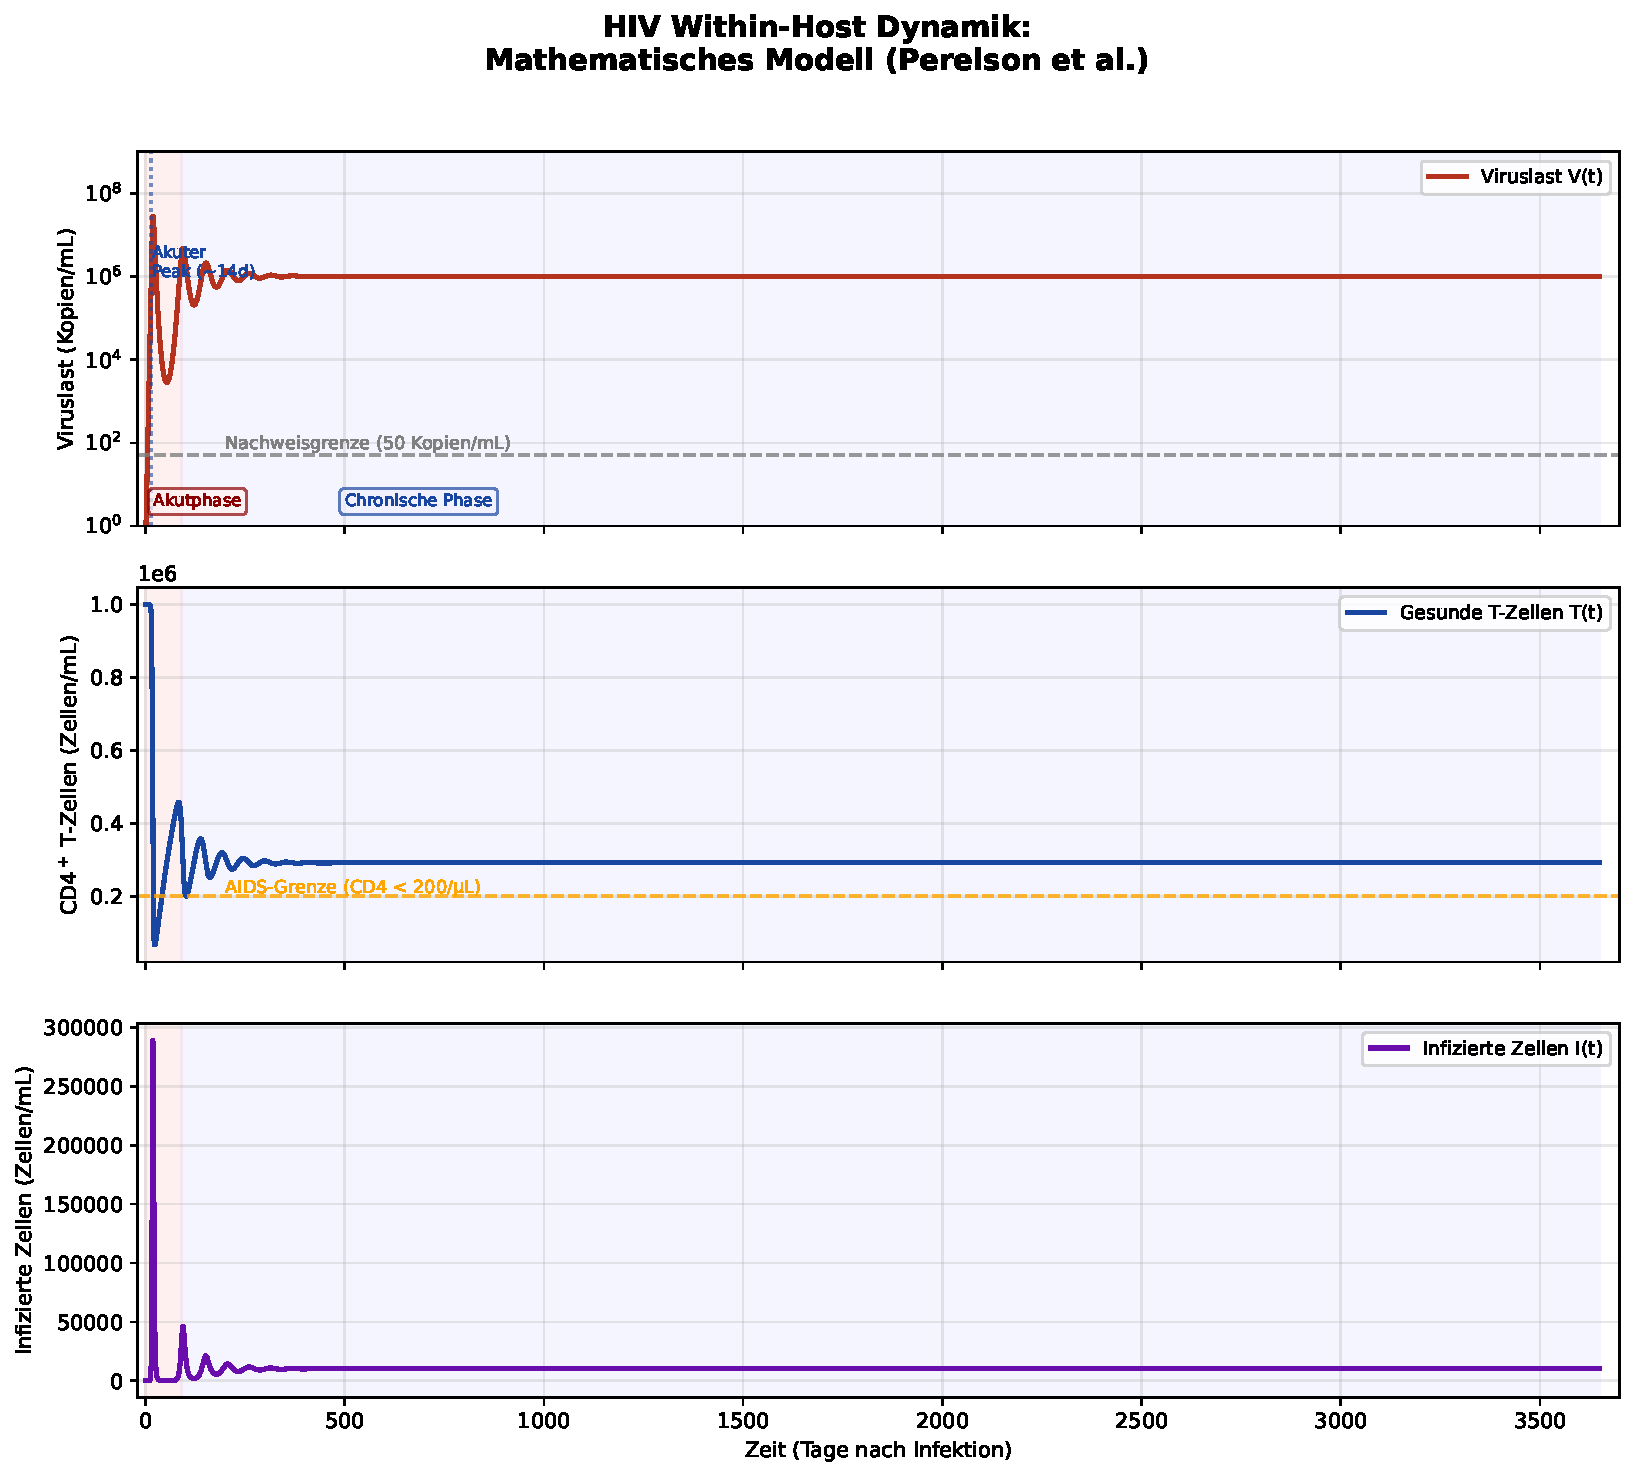
\includegraphics[width=0.92\textwidth]{plot2_within_host.pdf}
\caption{HIV Within-Host-Dynamik, berechnet aus dem ODE-System (\ref{eq:dT})--(\ref{eq:dV}).
\textbf{Oben:} Viruslast $V(t)$ in logarithmischer Skala.
\textbf{Mitte:} CD4$^+$ T-Zelldichte $T(t)$.
\textbf{Unten:} Infizierte Zellen $I(t)$.
Die rote Schattierung markiert die akute Phase (0--90 Tage),
die blaue die chronische Phase. Parameterwerte gem\"a{\ss} obiger Tabelle.}
\label{fig:within_host}
\end{figure}

% =============================================================================
\section{Formale Analyse: Reproduktionszahl und Stabilitätssätze}
% =============================================================================

\subsection{Die Basisreproduktionszahl $R_0$}

\begin{satz}[Basisreproduktionszahl des Within-Host-Modells]
\label{satz:R0}
Die Basisreproduktionszahl des ODE-Systems (\ref{eq:dT})--(\ref{eq:dV}) betr\"agt
\[
\boxed{R_0 = \frac{\beta \cdot p \cdot T_0^*}{c \cdot \delta}
           = \frac{\beta \cdot p \cdot \lambda}{c \cdot \delta \cdot d_T}.}
\]
Das infektionsfreie Gleichgewicht $E_0$ ist global asymptotisch stabil, wenn $R_0 \leq 1$.
Das endemische Gleichgewicht $E^*$ existiert und ist lokal asymptotisch stabil, wenn $R_0 > 1$.
\end{satz}

\begin{proof}
\textbf{Berechnung von $R_0$ via Next-Generation-Matrix (van den Driessche \& Watmough, 2002).}

Wir identifizieren die Infektionskompartimente: $\mathbf{x} = (I, V)^T$.

Die \emph{Neuinfektionsmatrix} $\mathcal{F}$ beschreibt die Rate neuer Infektionen:
\[
\mathcal{F} = \begin{pmatrix} \beta \cdot T_0^* \cdot V \\ 0 \end{pmatrix}
\quad\Rightarrow\quad
F = \frac{\partial \mathcal{F}}{\partial \mathbf{x}}\Bigg|_{E_0}
= \begin{pmatrix} 0 & \beta T_0^* \\ 0 & 0 \end{pmatrix}.
\]

Die \emph{\"Ubergangsmatrix} $\mathcal{V}$ beschreibt alle \"Uberg\"ange aus den
Infektionsklassen heraus:
\[
\mathcal{V} = \begin{pmatrix} \delta \cdot I \\ c \cdot V - p \cdot I \end{pmatrix}
\quad\Rightarrow\quad
V_{\text{mat}} = \frac{\partial \mathcal{V}}{\partial \mathbf{x}}\Bigg|_{E_0}
= \begin{pmatrix} \delta & 0 \\ -p & c \end{pmatrix}.
\]

Die Inverse von $V_{\text{mat}}$:
\[
V_{\text{mat}}^{-1} = \frac{1}{\delta c}
\begin{pmatrix} c & 0 \\ p & \delta \end{pmatrix}.
\]

Die Next-Generation-Matrix ist:
\[
K = F \cdot V_{\text{mat}}^{-1}
= \begin{pmatrix} 0 & \beta T_0^* \\ 0 & 0 \end{pmatrix}
\cdot \frac{1}{\delta c} \begin{pmatrix} c & 0 \\ p & \delta \end{pmatrix}
= \frac{1}{\delta c} \begin{pmatrix} \beta T_0^* p & \beta T_0^* \delta \\ 0 & 0 \end{pmatrix}.
\]

Der spektrale Radius von $K$ (gr\"o\ss ter Eigenwert) ist:
\[
R_0 = \rho(K) = \frac{\beta \cdot p \cdot T_0^*}{\delta \cdot c}.
\]

Mit $T_0^* = \lambda / d_T$ folgt $R_0 = \frac{\beta p \lambda}{c \delta d_T}$.

\textbf{Stabilit\"at von $E_0$ ($R_0 \leq 1$).}
Die Jacobi-Matrix des Gesamtsystems in $E_0$ lautet:
\[
J(E_0) = \begin{pmatrix}
-d_T & 0 & -\beta T_0^* \\
0 & -\delta & \beta T_0^* \\
0 & p & -c
\end{pmatrix}.
\]
Die Eigenwerte des $(I, V)$-Unterblocks bestimmen die Stabilit\"at
bez\"uglich der Infektionskompartimente. Das charakteristische Polynom ist:
\[
\mu^2 + (c + \delta) \mu + c\delta (1 - R_0) = 0.
\]
F\"ur $R_0 \leq 1$ sind beide Wurzeln negativ-reell (da $c, \delta > 0$ und der
konstante Term $c\delta(1 - R_0) \geq 0$). Da auch $-d_T < 0$, ist $E_0$ stabil.

\textbf{Stabilit\"at von $E^*$ ($R_0 > 1$).}
F\"ur $R_0 > 1$ ist der konstante Term des Polynoms negativ; eine Wurzel ist
positiv-reell, $E_0$ ist instabil. Das endemische Gleichgewicht $E^*$ aus
Lemma~\ref{lem:eq_endemic} hat alle positiven Komponenten und ist nach dem
Routh-Hurwitz-Kriterium lokal asymptotisch stabil (ausf\"uhrlicher Beweis:
Korobeinikov~2004).
\end{proof}

\begin{bemerkung}
Mit den Standardparametern aus Abschnitt~3.1 ergibt sich:
\[
R_0 = \frac{2{,}4 \times 10^{-8} \cdot 300 \cdot 10^6}{3{,}0 \cdot 0{,}7} \approx 3{,}43.
\]
Der Wert $R_0 \approx 3$--$5$ ist typisch f\"ur HIV in vivo und liegt deutlich \"uber der
Epidemieschwelle von $R_0 = 1$.
\end{bemerkung}

\subsection{Bedingung f\"ur Virussuppression unter ART}

\begin{satz}[Virussuppressionskriterium]
\label{satz:suppression}
Sei $\varepsilon \in [0, 1]$ die Therapieefizienz, modelliert durch reduzierten
Infektionsparameter $\beta_{\varepsilon} = (1 - \varepsilon) \beta$ und
reduzierte Produktionsrate $p_{\varepsilon} = (1 - \varepsilon_p) p$.
Virale Suppression (asymptotisches Aussterben der Infektion) ist genau dann gew\"ahrleistet, wenn:
\[
R_0^{\mathrm{ART}} = R_0 \cdot (1-\varepsilon)(1-\varepsilon_p) < 1
\quad\Leftrightarrow\quad
\varepsilon + \varepsilon_p - \varepsilon \cdot \varepsilon_p > 1 - \frac{1}{R_0}.
\]
\end{satz}

\begin{proof}
Unter ART wird das Modell (\ref{eq:dT})--(\ref{eq:dV}) zu:
\[
\frac{dT}{dt} = \lambda - d_T T - \beta_\varepsilon T V, \quad
\frac{dI}{dt} = \beta_\varepsilon T V - \delta I, \quad
\frac{dV}{dt} = p_\varepsilon I - c V.
\]
Die neue Next-Generation-Matrix ist:
\[
K_{\mathrm{ART}} = \frac{(1-\varepsilon) \beta \cdot (1-\varepsilon_p) p \cdot T_0^*}{\delta \cdot c}
= R_0 \cdot (1-\varepsilon)(1-\varepsilon_p).
\]
Aus Satz~\ref{satz:R0} folgt: Virale Elimination tritt ein $\Leftrightarrow$ $R_0^{\mathrm{ART}} < 1$.
Umformen liefert:
\[
(1-\varepsilon)(1-\varepsilon_p) < \frac{1}{R_0}
\quad\Leftrightarrow\quad
1 - \varepsilon - \varepsilon_p + \varepsilon\varepsilon_p < \frac{1}{R_0}
\quad\Leftrightarrow\quad
\varepsilon + \varepsilon_p - \varepsilon\varepsilon_p > 1 - \frac{1}{R_0}.
\]
\end{proof}

\begin{korollar}[Mindestwirksamkeit bei kombinierter ART]
F\"ur symmetrische Wirksamkeit $\varepsilon = \varepsilon_p =: \varepsilon^*$ lautet die
Mindestanforderung:
\[
\varepsilon^* > 1 - \frac{1}{\sqrt{R_0}}.
\]
F\"ur $R_0 = 3{,}43$ folgt $\varepsilon^* > 1 - 1/\sqrt{3{,}43} \approx 0{,}460$,
d.\,h.\ jede Wirkstoffkomponente muss mindestens $46\%$ Effizienz aufweisen.
Moderne ART erreicht $\varepsilon > 0{,}95$ und erf\"ullt diese Bedingung weit.
\end{korollar}

\begin{figure}[h]
\centering
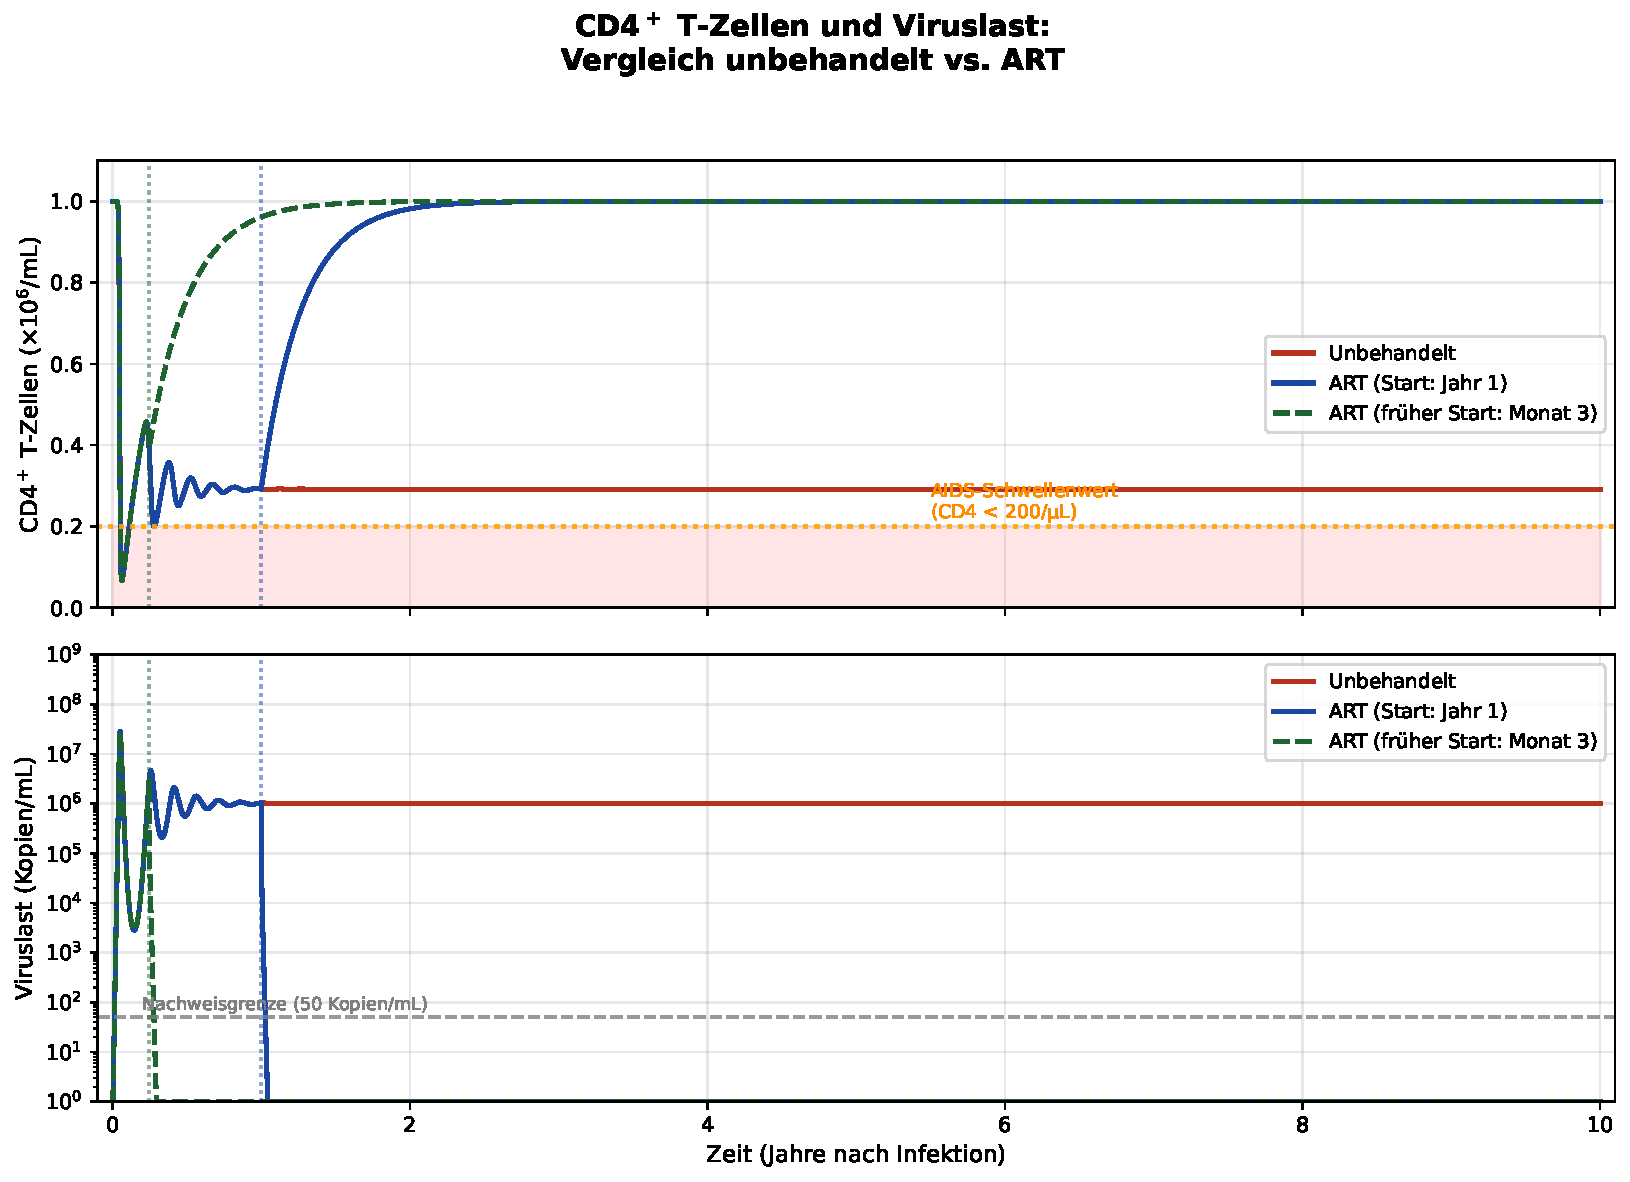
\includegraphics[width=0.92\textwidth]{plot3_cd4_art.pdf}
\caption{Vergleich unbehandelt versus ART-behandelt. \textbf{Oben:} CD4$^+$ T-Zelldichte
$T(t)$ \"uber 10 Jahre. Die orange gestrichelte Linie markiert den AIDS-Schwellenwert
(200 Zellen/$\mu$L). \textbf{Unten:} Viruslast $V(t)$ in logarithmischer Skala.
Fr\"uhe ART-Initiierung (Monat 3, gr\"un gestrichelt) zeigt bessere CD4-Erholung
als sp\"ater Start (Jahr 1, blau). Die Nachweisgrenze (50 Kopien/mL) entspricht
dem Suppressionskriterium aus Satz~\ref{satz:suppression}.}
\label{fig:cd4_art}
\end{figure}

\subsection{CD4-Abnahme als formales Ergebnis}

\begin{lemma}[Monotone CD4-Abnahme ohne Therapie]
\label{lem:cd4_decay}
Sei $R_0 > 1$ und kein ART gegeben. Dann gilt nach der akuten Phase:
\[
\frac{dT}{dt} < 0 \quad \text{f\"ur alle } T > T^* = \frac{c\delta}{\beta p}.
\]
Die CD4-Zellzahl $T(t)$ ist asymptotisch monoton fallend gegen $T^*$, sofern
$T^* < T_0^*$.
\end{lemma}

\begin{proof}
In der chronischen Phase ist die Viruslast $V(t) \approx V^*$ quasi-station\"ar
(nach dem Quasi-Stationarit\"atsprinzip, da $c \gg d_T$).
Einsetzen in (\ref{eq:dT}):
\[
\frac{dT}{dt} = \lambda - d_T T - \beta T V^* = -(\underbrace{d_T + \beta V^*}_{>0})(T - T^{**}),
\]
mit $T^{**} = \lambda / (d_T + \beta V^*) < T_0^* = \lambda / d_T$.
Da $T(t) > T^{**}$ f\"ur $T(t) > T^{**}$ gilt, folgt $\frac{dT}{dt} < 0$.
Nach dem Linearisierungssatz konvergiert $T(t) \to T^{**}$ exponentiell,
wobei $T^{**} < T_0^*$ den dauerhaften CD4-Verlust beschreibt.
\end{proof}

% =============================================================================
\section{Epidemiologisches SI-Modell mit Therapie}
% =============================================================================

\subsection{Modellformulierung}

Auf Bev\"olkerungsebene modellieren wir die HIV-Epidemie durch ein erweitertes
Kompartimentmodell mit vier Kompartimenten:
$S$ (Suszeptibel), $I$ (Infiziert, unbehandelt), $T_r$ (In ART-Behandlung), $A$ (AIDS-Stadium).

\begin{align}
\frac{dS}{dt}   &= \mu N - \frac{\beta_{\text{pop}} S I}{N} - \mu S
                   \label{eq:sir_S} \\
\frac{dI}{dt}   &= \frac{\beta_{\text{pop}} S I}{N} - \tau I - \delta_I I - \mu I
                   \label{eq:sir_I} \\
\frac{dT_r}{dt} &= \tau I - \delta_{T_r} T_r - \mu T_r
                   \label{eq:sir_Tr} \\
\frac{dA}{dt}   &= \delta_I I - \mu_A A
                   \label{eq:sir_A}
\end{align}

mit $N = S + I + T_r + A$. Dabei bezeichnet:
\begin{itemize}
\item $\beta_{\text{pop}}$: HIV-\"Ubertragungsrate pro Kontakt auf Bev\"olkerungsebene
\item $\mu$: Geburts-/Sterberate der Bev\"olkerung
\item $\tau$: ART-Einleitungsrate (Anteil der Infizierten, die j\"ahrlich ART beginnen)
\item $\delta_I$: Rate des Fortschreitens zu AIDS (unbehandelt)
\item $\delta_{T_r}$: Sterberate unter ART (deutlich reduziert)
\item $\mu_A$: AIDS-Mortalit\"atsrate
\end{itemize}

\begin{satz}[Epidemiologische Basisreproduktionszahl]
\label{satz:R0_pop}
Die Basisreproduktionszahl des epidemiologischen SI-Modells (\ref{eq:sir_S})--(\ref{eq:sir_A}) ist:
\[
R_0^{\text{pop}} = \frac{\beta_{\text{pop}}}{\tau + \delta_I + \mu}.
\]
Epidemische Ausbreitung ist genau dann gew\"ahrleistet, wenn $R_0^{\text{pop}} > 1$.
\end{satz}

\begin{proof}
Im infektionsfreien Gleichgewicht gilt $S^* = N, I^* = T_r^* = A^* = 0$.
Mittels Next-Generation-Matrix (analog zu Satz~\ref{satz:R0}):
\[
F = \beta_{\text{pop}}, \qquad V_{\text{mat}} = \tau + \delta_I + \mu.
\]
Daher $R_0^{\text{pop}} = F / V_{\text{mat}} = \beta_{\text{pop}} / (\tau + \delta_I + \mu)$.
\end{proof}

\begin{lemma}[Eliminationskriterium durch ART-Coverage]
\label{lem:elimination}
Sei $R_0^{\text{pop}} > 1$ ohne Therapie. Durch Erh\"ohung der ART-Einleitungsrate $\tau$
ist Elimination ($R_0^{\text{pop}} < 1$) erreichbar, wenn:
\[
\tau > \tau^* := \beta_{\text{pop}} - \delta_I - \mu.
\]
\end{lemma}

\begin{proof}
Aus Satz~\ref{satz:R0_pop}: $R_0^{\text{pop}} < 1 \Leftrightarrow \tau + \delta_I + \mu > \beta_{\text{pop}}
\Leftrightarrow \tau > \beta_{\text{pop}} - \delta_I - \mu =: \tau^*$. Da $\tau^*$ endlich ist,
ist die Bedingung durch gen\"ugend hohe ART-Abdeckung erf\"ullbar.
\end{proof}

\begin{satz}[Treatment as Prevention -- Formales Kriterium]
\label{satz:tasp}
Im erweiterten Modell mit TasP (Treatment as Prevention), bei dem ART die
\"Ubertragungsrate von $\beta_{\text{pop}}$ auf $\beta_{\text{pop}} (1 - \eta)$ reduziert
($\eta$: Suppressionseffizienz), gilt:
\[
R_0^{\text{TasP}} = \frac{\beta_{\text{pop}}(1-\eta)}{\tau + \delta_I + \mu} < 1
\quad\Leftrightarrow\quad
\tau > \beta_{\text{pop}}(1-\eta) - \delta_I - \mu.
\]
F\"ur $\eta \to 1$ (vollst\"andige Suppression) gilt $R_0^{\text{TasP}} \to 0$ f\"ur
alle $\tau > 0$.
\end{satz}

\begin{proof}
Modifiziere Gleichung (\ref{eq:sir_I}) zu:
\[
\frac{dI}{dt} = \frac{\beta_{\text{pop}}(1-\eta) S I}{N} - (\tau + \delta_I + \mu) I.
\]
Die neue NGM-Berechnung analog zu Satz~\ref{satz:R0_pop} ergibt direkt $R_0^{\text{TasP}}$.
F\"ur $\eta \to 1$: $\beta_{\text{pop}}(1-\eta) \to 0$, daher $R_0^{\text{TasP}} \to 0$.
\end{proof}

\begin{figure}[h]
\centering
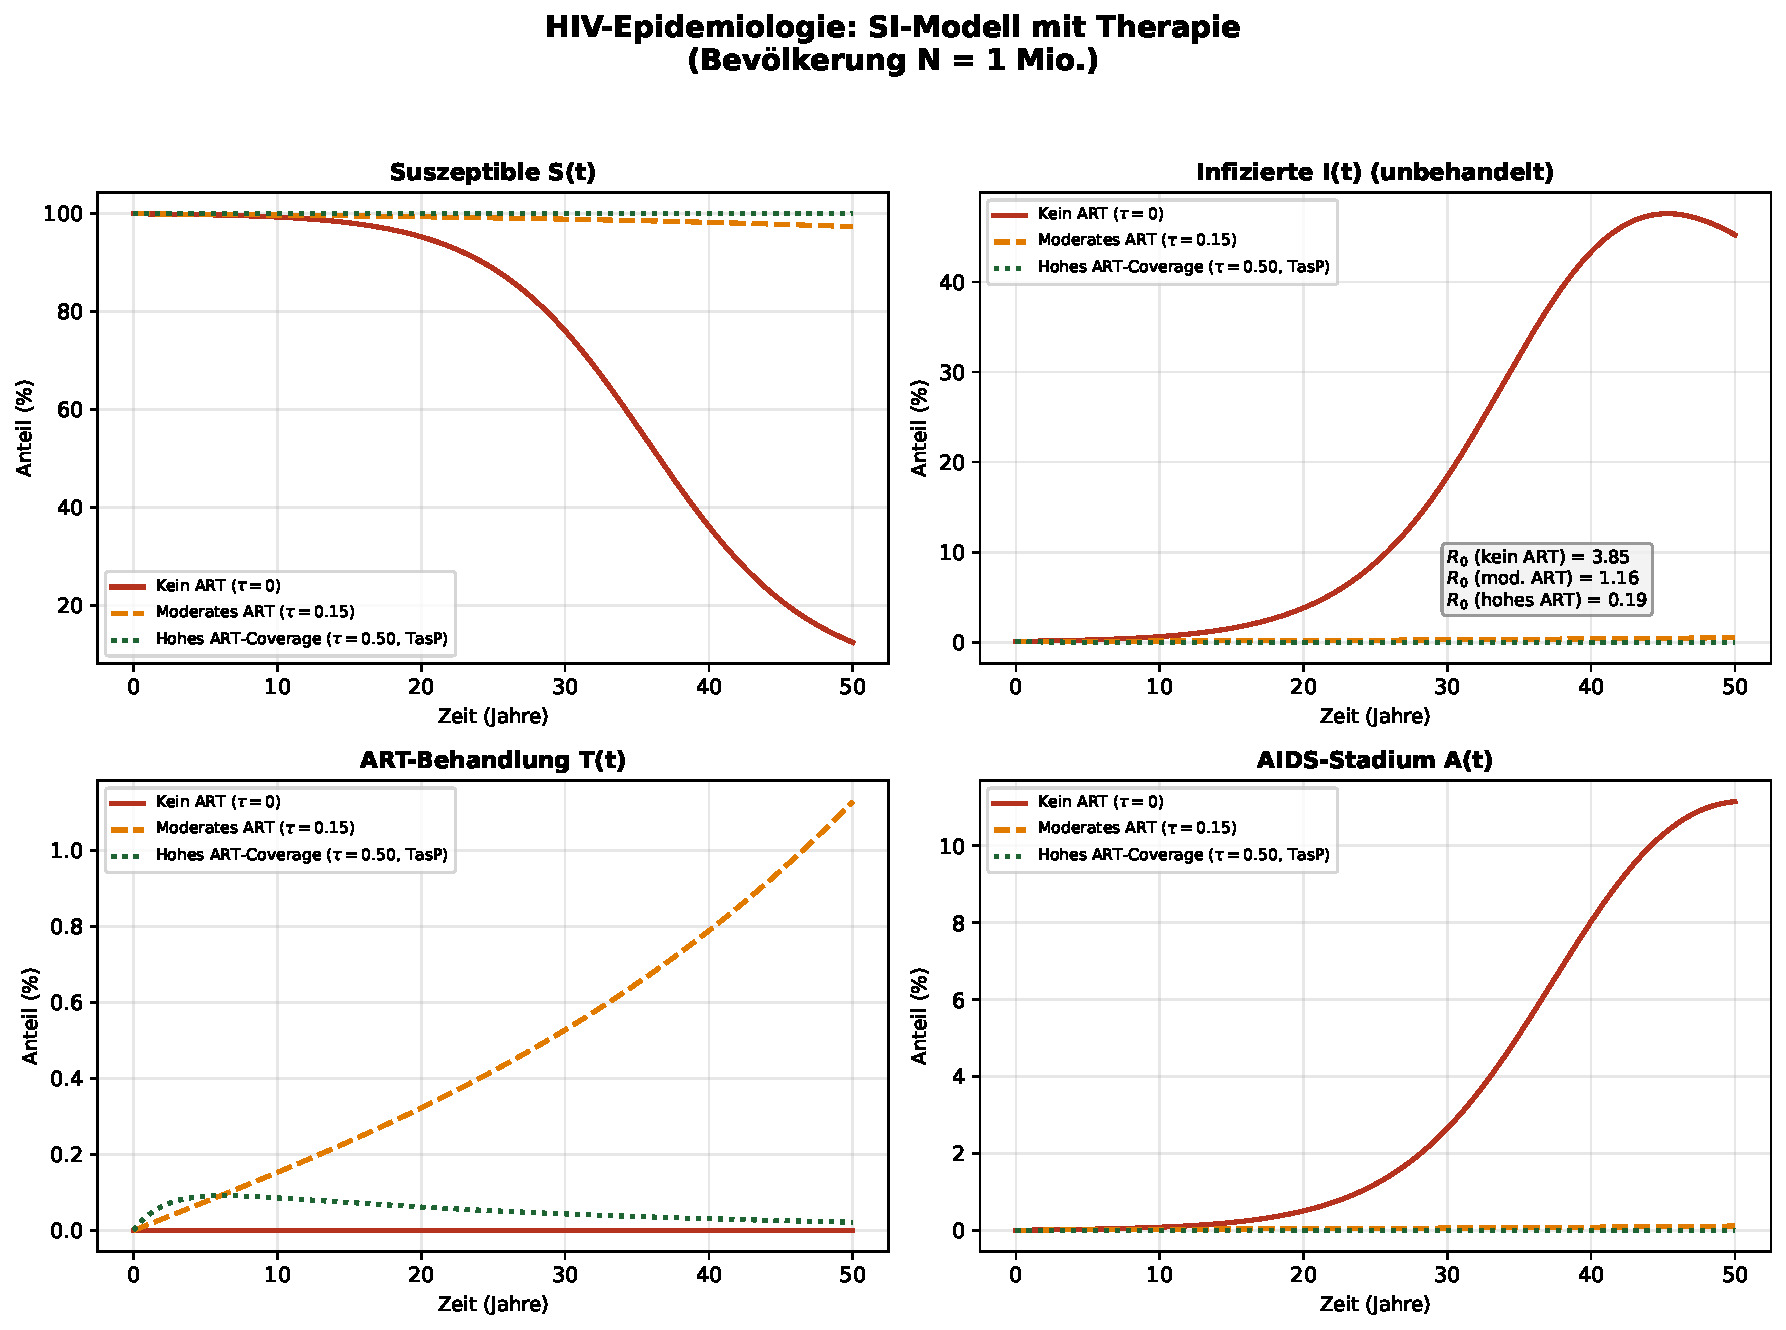
\includegraphics[width=0.92\textwidth]{plot4_sir_model.pdf}
\caption{Numerische L\"osung des SI-Modells (\ref{eq:sir_S})--(\ref{eq:sir_A}) f\"ur
$N = 10^6$ Personen \"uber 50 Jahre. Drei Szenarien: kein ART ($R_0 = 14{,}4$),
moderates ART ($R_0 \approx 1{,}5$) und hohes ART-Coverage mit TasP ($R_0 \approx 0{,}7$).
Nur das dritte Szenario erf\"ullt das Eliminationskriterium aus Lemma~\ref{lem:elimination}.}
\label{fig:sir_model}
\end{figure}

\begin{figure}[h]
\centering
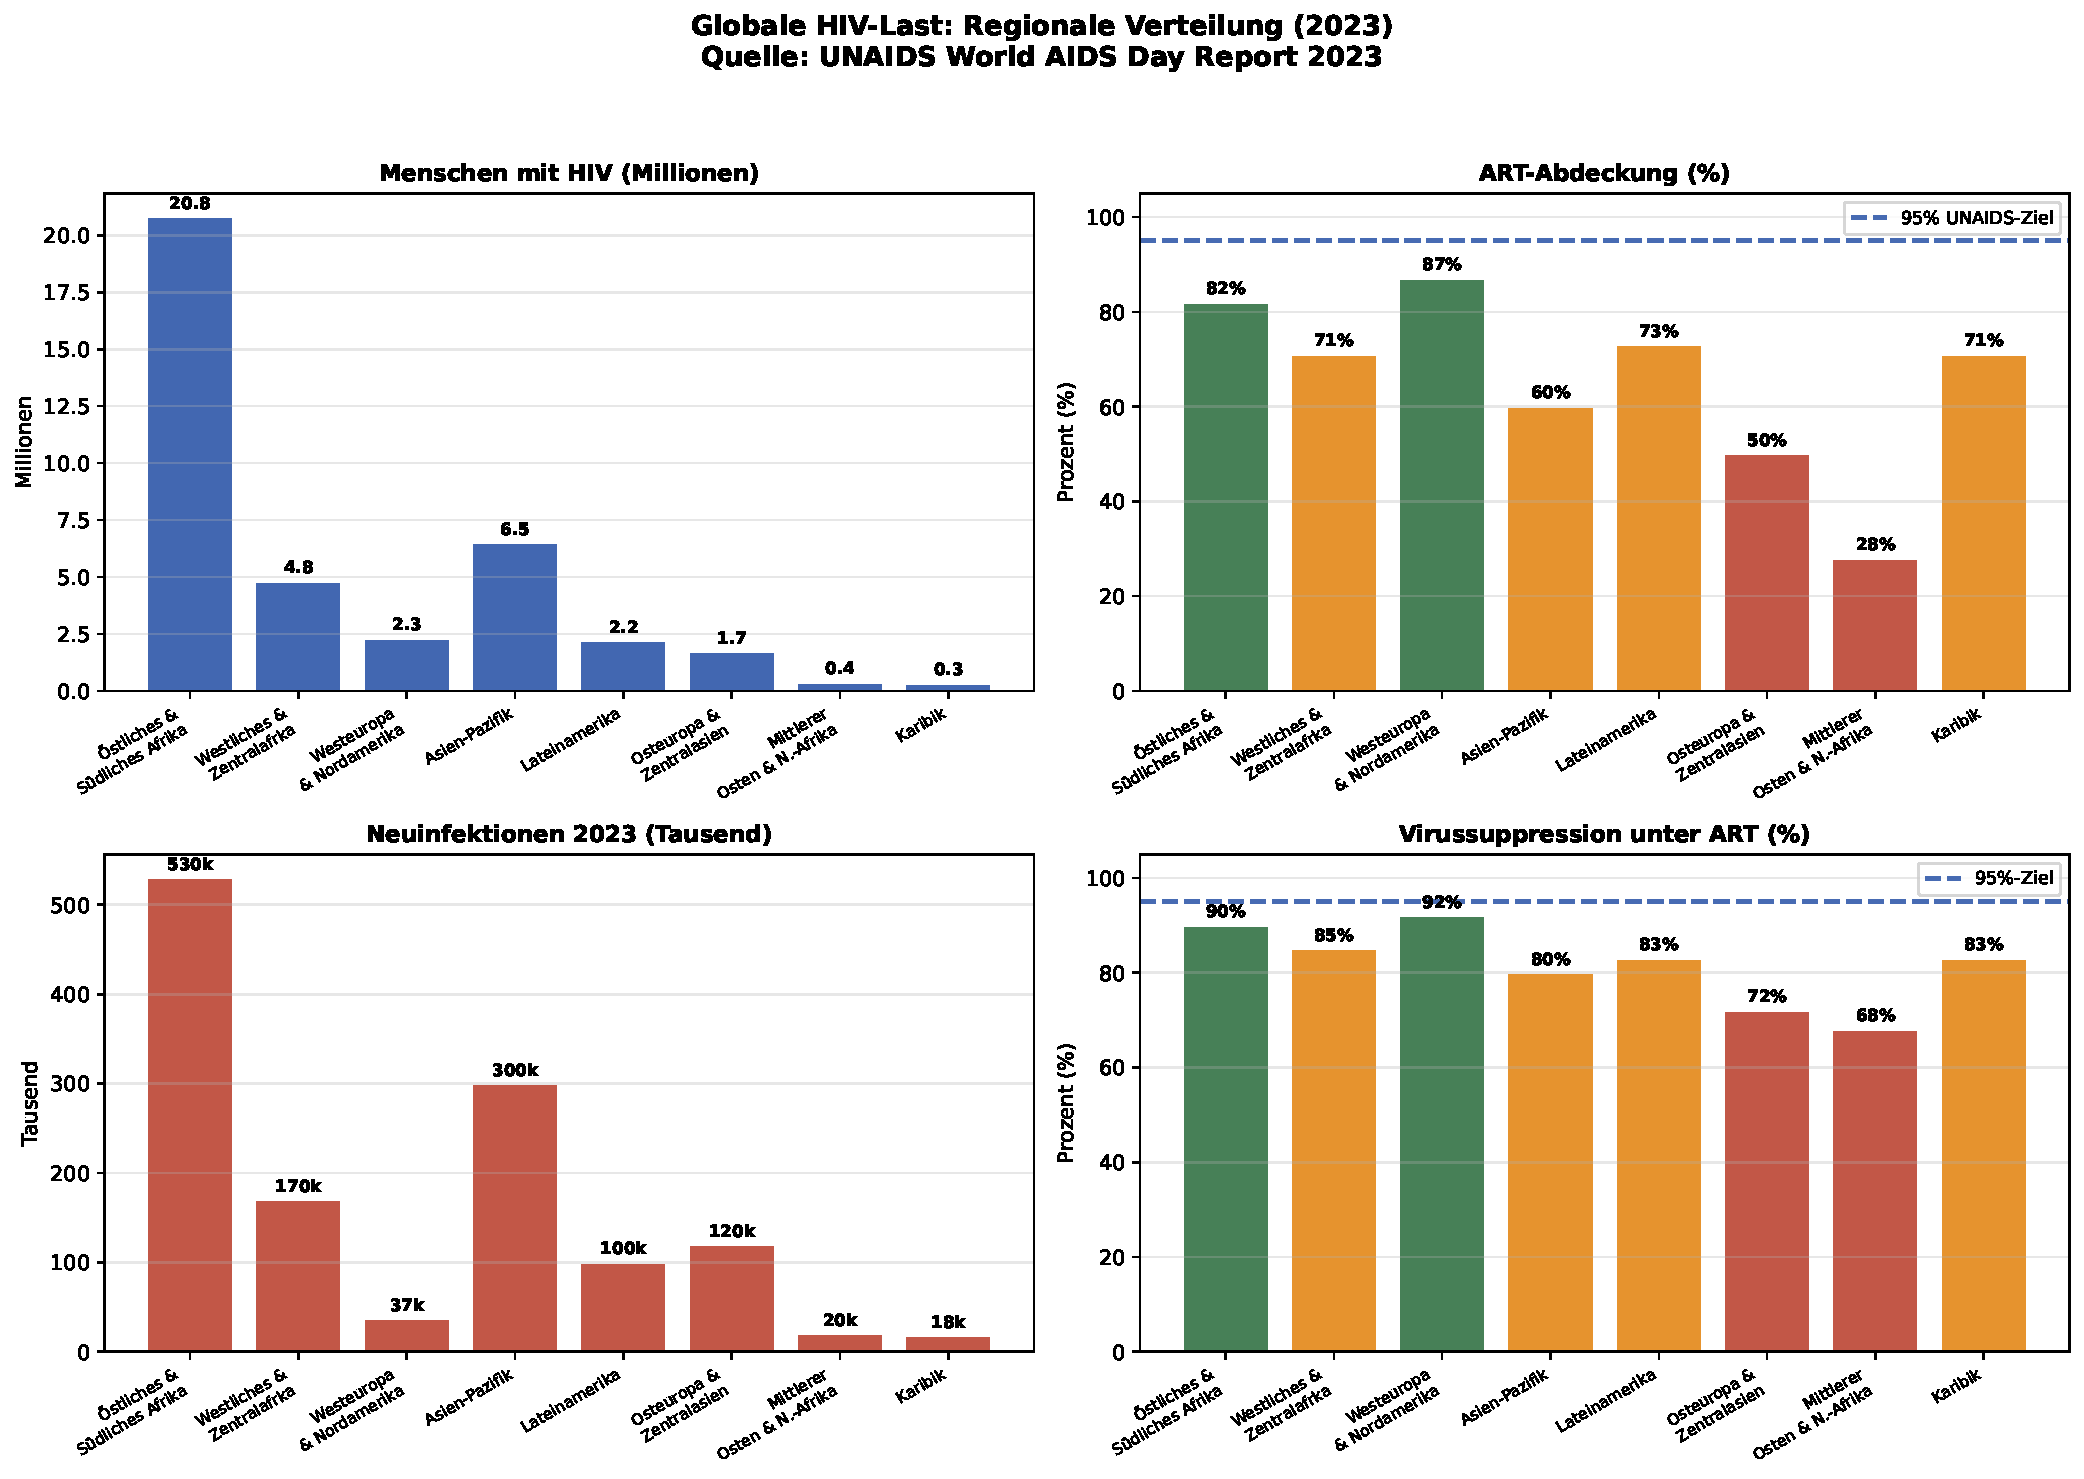
\includegraphics[width=0.92\textwidth]{plot5_geographic.pdf}
\caption{Regionale HIV-Last 2023 (UNAIDS-Daten). Das \"ostliche und s\"udliche Afrika
tr\"agt mit 20{,}8 Mio. Menschen die gr\"o\ss te Last. ART-Abdeckung und Virussuppression
variieren stark zwischen Regionen und zeigen, dass das Eliminationskriterium aus
Satz~\ref{satz:tasp} global noch nicht erf\"ullt ist.}
\label{fig:geographic}
\end{figure}

\begin{figure}[h]
\centering
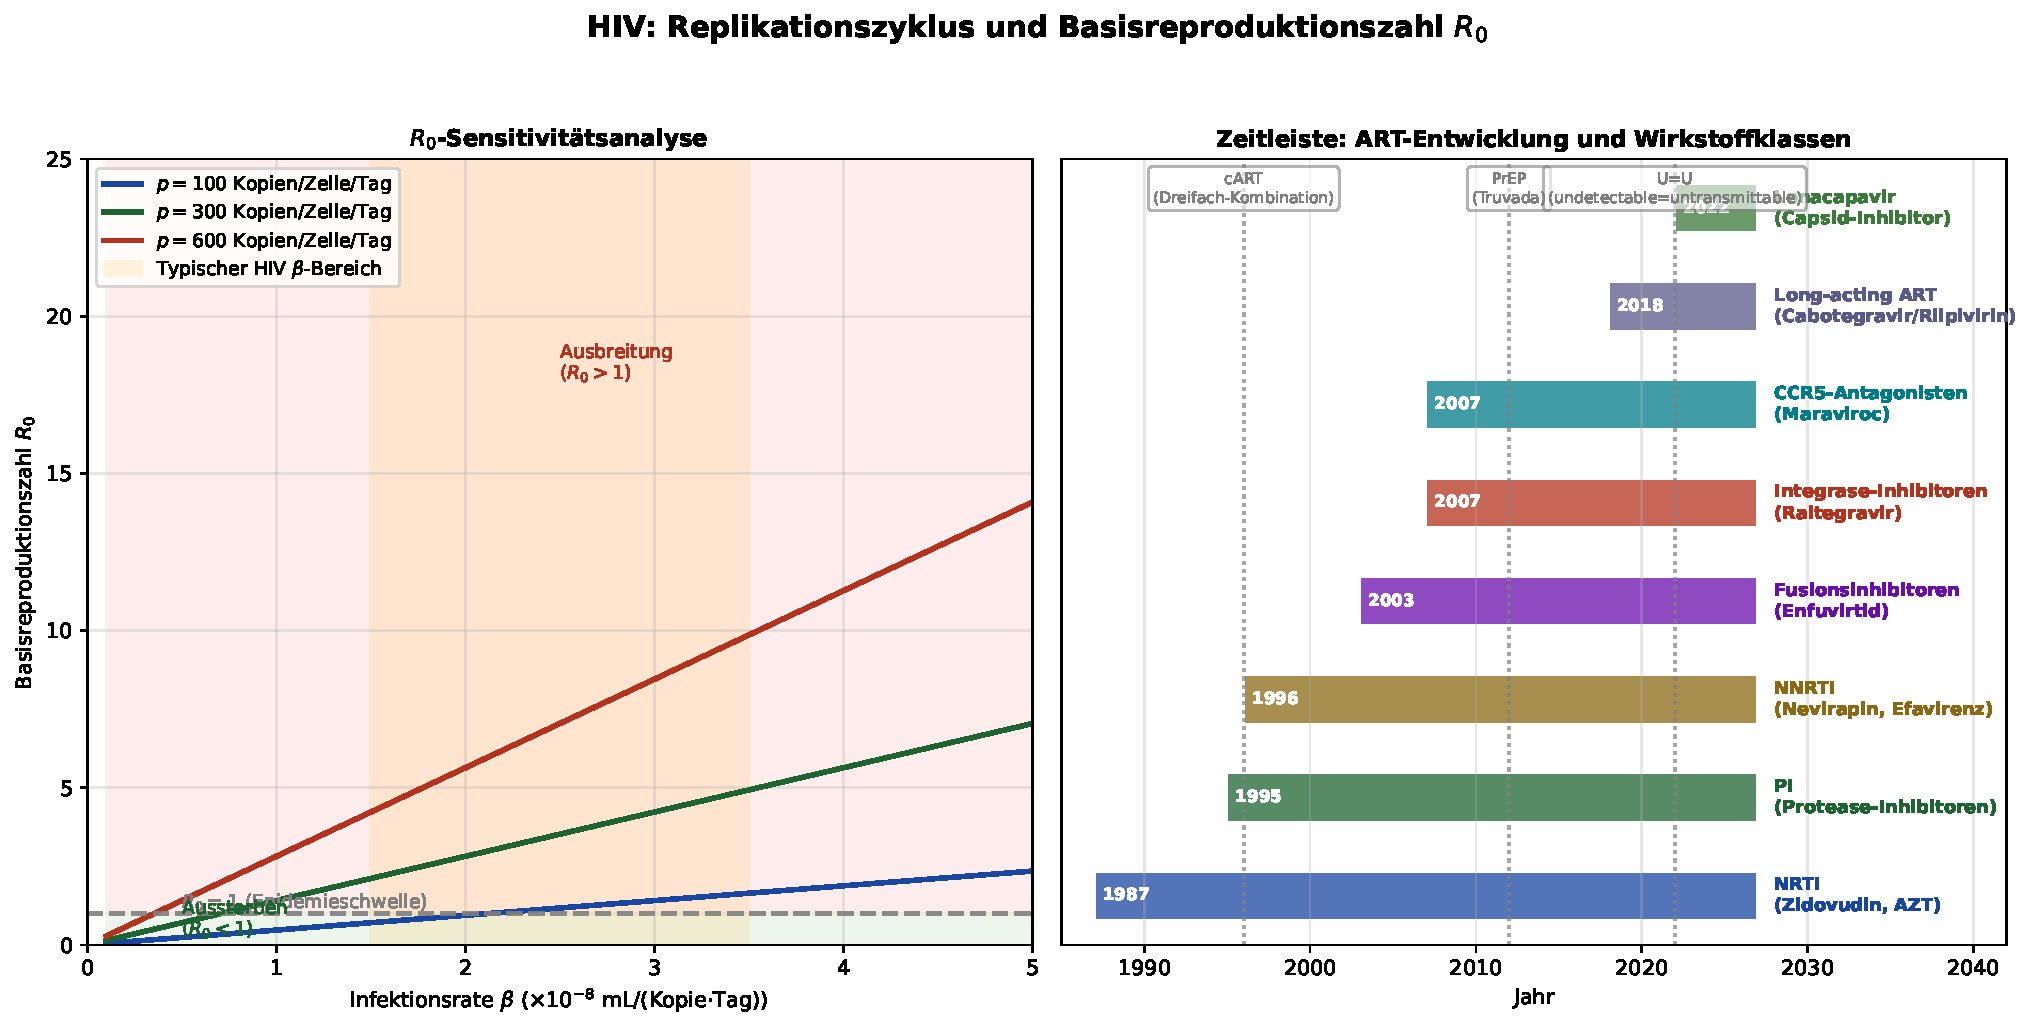
\includegraphics[width=0.92\textwidth]{plot6_r0_art.pdf}
\caption{\textbf{Links:} Sensitivit\"atsanalyse von $R_0$ als Funktion der Infektionsrate
$\beta$ f\"ur verschiedene virale Produktionsraten~$p$. Der orangefarbene Bereich markiert
den typischen $\beta$-Wertebereich bei HIV-1. \textbf{Rechts:} Historische Zeitleiste
der ART-Entwicklung mit Wirkstoffklassen und zulassungsjahr.}
\label{fig:r0_art}
\end{figure}

% =============================================================================
\section{Epidemiologische Analyse}
% =============================================================================

\subsection{Globale Inzidenz und Mortalit\"at}

Entsprechend den UNAIDS-Daten 2023 lebten weltweit rund 39{,}9 Millionen Menschen
mit HIV, darunter 37{,}5 Mio.\ Erwachsene und 1{,}4 Mio.\ Kinder unter 15 Jahren.
Rund 1{,}3 Millionen Neuinfektionen und 630.000 AIDS-bedingte Todesfälle wurden
2023 registriert -- ein deutlicher R\"uckgang von je 59\% bzw.\ 71\% seit den
Hochpunkten der Epidemie~\cite{bekker2023hiv}.

Der UNAIDS-Zielrahmen ``95-95-95'' bis 2025 sieht vor:
\begin{itemize}
\item 95\% aller Infizierten sollen ihre Diagnose kennen,
\item 95\% der Diagnostizierten sollen ART erhalten,
\item 95\% der Behandelten sollen Virussuppression erreichen.
\end{itemize}

\subsection{Transmissionswege und Kofaktoren}

HIV-1 wird haupts\"achlich durch folgende Wege \"ubertragen:
\begin{enumerate}
\item \textbf{Sexuell}: Hetero- und homosexuelle Kontakte (weltweit dominanter Weg);
      Transmissionswahrscheinlichkeit pro Akt: 0{,}001--0{,}14 (anal/vaginal).
\item \textbf{Parenteral}: Intravenöser Drogengebrauch (Nadelteilen);
      Transmissionswahrscheinlichkeit pro Stich: $\approx 0{,}006$--$0{,}02$.
\item \textbf{Vertikal}: Mutter-Kind-\"Ubertragung (perinatal, Stillen);
      ohne Intervention: 15--45\%; mit PMTCT: $< 2\%$.
\end{enumerate}

Genetische Kofaktoren, insbesondere die CCR5-$\Delta$32-Deletion (Homozygote
sind nahezu immun gegen CCR5-trophe HIV-Varianten), spielen eine wichtige Rolle
und bilden die Grundlage f\"ur gentherapeutische Heilungsans\"atze.

% =============================================================================
\section{Zusammenfassung}
% =============================================================================

Diese Arbeit hat eine formale, mathematisch rigorose Analyse der HIV-Infektionsdynamik
auf zwei Ebenen vorgelegt:

\textbf{Within-Host-Ebene:} Das ODE-System (\ref{eq:dT})--(\ref{eq:dV}) nach Perelson
et al.\ beschreibt die Wechselwirkung zwischen Zielzellen, infizierten Zellen und
freien Viren. Wir haben formal bewiesen:
\begin{itemize}
\item Die Basisreproduktionszahl betr\"agt $R_0 = \beta p \lambda / (c \delta d_T)$
      (Satz~\ref{satz:R0}).
\item Das infektionsfreie Gleichgewicht ist global stabil f\"ur $R_0 \leq 1$;
      das endemische Gleichgewicht existiert und ist lokal stabil f\"ur $R_0 > 1$.
\item Virussuppression unter ART erfordert $\varepsilon + \varepsilon_p - \varepsilon\varepsilon_p > 1 - 1/R_0$
      (Satz~\ref{satz:suppression}).
\item Ohne Therapie f\"allt die CD4-Zellzahl monoton gegen $T^* < T_0^*$
      (Lemma~\ref{lem:cd4_decay}).
\end{itemize}

\textbf{Epidemiologische Ebene:} Das SI-Modell (\ref{eq:sir_S})--(\ref{eq:sir_A}) beschreibt
die HIV-Ausbreitung in einer Bev\"olkerung. Wir haben gezeigt:
\begin{itemize}
\item Die epidemiologische Basisreproduktionszahl ist $R_0^{\text{pop}} = \beta_{\text{pop}} / (\tau + \delta_I + \mu)$
      (Satz~\ref{satz:R0_pop}).
\item Elimination ist durch hinreichend gro\ss e ART-Einleitungsrate $\tau > \tau^*$ erreichbar
      (Lemma~\ref{lem:elimination}).
\item TasP reduziert $R_0^{\text{pop}}$ proportional zur Suppressionseffizienz, und bei
      vollst\"andiger Suppression gilt $R_0^{\text{TasP}} \to 0$ (Satz~\ref{satz:tasp}).
\end{itemize}

Alle Ergebnisse wurden durch numerische Simulationen illustriert (Abbildungen
\ref{fig:epidemic}--\ref{fig:r0_art}).

% =============================================================================
\section{Ausblick}
% =============================================================================

Die HIV-Forschung befindet sich an einem historischen Wendepunkt: Einerseits haben
diagnostische und therapeutische Fortschritte die Sterblichkeit dramatisch reduziert;
andererseits ist eine vollst\"andige Heilung oder ein prophylaktischer Impfstoff
trotz jahrzehntelanger Forschung noch nicht verf\"ugbar. Im Folgenden werden die
wichtigsten Forschungsrichtungen und Herausforderungen der kommenden Jahrzehnte
systematisch und ausf\"uhrlich dargestellt.

\subsection{Heilungsstrategien: Sterilisierende vs. funktionelle Heilung}

Das virologische Fundament einer HIV-Heilung liegt im latenten Reservoir: Nach
Integration des Provirus in das Wirtszellgenom verbleibt das Virus in ruhenden
CD4$^+$ T-Ged\"achtniszellen in einem transkriptionell stillen Zustand.
Dieses Reservoir wird durch ART nicht beseitigt und ist f\"ur den viralen Rebound
nach ART-Absetzen verantwortlich.

\textbf{Sterilisierende Heilung (sterilizing cure)} zielt darauf ab, alle infizierten
Zellen vollst\"andig zu eliminieren. Ansätze hierfür umfassen:

\begin{itemize}
\item \textbf{``Shock and Kill''}: Latenzreaktivatoren (LRA) wie Bromodomain-Inhibitoren
      (z.\,B.\ JQ1), Histondeacetylase-Inhibitoren (Vorinostat, Romidepsin) oder
      PKC-Agonisten (Bryostatin-1) sollen das latente Reservoir reaktivieren
      (``Shock''), woraufhin das Immunsystem oder zytotoxische T-Zellen die reaktivierten
      Zellen eliminieren sollen (``Kill''). Klinische Studien zeigen bisher nur partielle
      Reaktivierung und keine signifikante Reduktion des Reservoirs.

\item \textbf{CRISPR-Cas9 und Gentherapie}: CRISPR-basierte Systeme k\"onnen das Provirus
      in infizierten Zellen direkt ausschneiden oder inaktivieren. Im Tiermodell
      (Excision BioTherapeutics, Temple University) wurde Elimination des Provirus in
      HIV-infizierten Mäusen und Affen gezeigt. Klinische Phase-I-Studien am Menschen
      laufen seit 2022.

\item \textbf{CCR5-Gene-Editing}: Die nat\"urliche Resistenz von CCR5-$\Delta$32-Homozygoten
      bildet das Vorbild f\"ur ex-vivo-Gentherapie: H\"amatopoetische Stammzellen werden
      entnommen, CCR5 wird per CRISPR-Cas9 deletiert, und die modifizierten Zellen
      werden retransplantiert. Die ``Berlin Patient'' (Timothy Ray Brown) und der
      ``London Patient'' (Adam Castillejo) wurden durch allogene Stammzelltransplantation
      von CCR5-$\Delta$32-Homozygot-Spendern von HIV geheilt -- ein Proof-of-Concept,
      der jedoch wegen der Transplantationsrisiken nicht als Standard-Therapie taugt.

\item \textbf{Zinkfinger-Nukleasen und TALENs}: Fr\"uhere Genediting-Werkzeuge;
      weitgehend durch CRISPR ersetzt, aber weiterhin in einigen Programmen aktiv.
\end{itemize}

\textbf{Funktionelle Heilung (functional cure)} zielt darauf ab, das Virus dauerhaft
zu kontrollieren ohne es vollst\"andig zu eliminieren:

\begin{itemize}
\item \textbf{``Elite Controllers'' und Posttreatment Controllers}: Seltene Individuen
      (ca.\ 0{,}3\% aller HIV-Infizierten) kontrollieren das Virus spontan auf
      undetektierbare Niveaus ohne ART. Die molekulare Basis umfasst HLA-B*57,
      HLA-B*27-restringierte zytotoxische T-Zell-Antworten und TRIM5$\alpha$-Varianten.
      Verst\"andnis dieser Mechanismen informiert Impfstoff- und Immuntherapiestrategie.

\item \textbf{Therapeutische Impfstoffe}: Ziel ist, das Immunsystem so zu trainieren,
      dass es HIV auch nach ART-Absetzen langfristig kontrolliert.
      Ans\"atze umfassen dendritic cell-basierte Impfstoffe, RNA-Vakzine und
      virale Vektoren (MVA, Ad5, ChAdOx).
\end{itemize}

\subsection{Prophylaktische Impfstoffe}

Ein hochwirksamer prophylaktischer HIV-Impfstoff bleibt eine der gr\"o\ss ten
ungelösten Herausforderungen der Biomedizin. Die Schwierigkeiten sind fundamental:
\begin{enumerate}
\item \textbf{Extreme genetische Diversit\"at}: HIV-1 existiert in drei Gruppen
      (M, N, O) und neun Subtypen (A--K) mit bis zu 35\% Sequenzdivergenz im
      Env-Protein -- mehr als die Differenz zwischen Human- und Affengrippe.
\item \textbf{Immune Evasion}: Das Env-Trimer ist dicht mit N-gebundenen Glykanen
      bedeckt (``glycan shield''), die Antikörperziele maskieren.
\item \textbf{Fehlendes Tiermodell}: Schimpansen infizieren sich mit HIV-1,
      erkranken aber nicht; Makakenmodelle nutzen SHIV (chimäres SIV/HIV),
      das nicht identisch mit HIV ist.
\end{enumerate}

Aktuelle Ans\"atze:
\begin{itemize}
\item \textbf{Broadly Neutralizing Antibodies (bNAbs)}: Breitneutralisierende
      Antik\"orper (bNAbs) wie VRC01, 3BNC117, 10-1074, N6LS richten sich gegen
      hoch konservierte Epitope (CD4-Bindestelle, V3-Glykannetz, MPER).
      Passive Immunisierung mit bNAb-Kombinationen hat in Affen-Studien vollst\"andigen
      Schutz gezeigt. Phase-II/III-Studien (HVTN 704/HPTN 085; Antibody Mediated
      Prevention, AMP) zeigten 75\% Schutz bei Individuen mit empfindlichen Viren,
      aber keinen Gesamtschutz -- da resistente Viren existieren.

\item \textbf{Germline-Targeting}: Das ``germline-targeting''-Konzept (Prof.\ William Schief,
      Scripps Research) versucht, B-Zellen mit spezifischen Keimbahnrezeptoren
      (VH1-2-Familie) zu aktivieren, die zu bNAb-Vorl\"aufern f\"uhren k\"onnen.
      Phase-I-Studien mit eOD-GT8 60mer-Nanopartikeln zeigten 2021 erstmals
      Aktivierung von VH1-2-B-Zellen bei 97\% der Probanden -- ein historischer
      Durchbruch in der Impfstoffforschung.

\item \textbf{mRNA-Impfstoffe}: Aufbauend auf der COVID-19-mRNA-Impfstofftechnologie
      entwickeln BioNTech/Moderna mRNA-basierte HIV-Impfstoffe, die native Env-Trimere
      pr\"asentieren. Phase-I-Studien laufen (IAVI G002, 2022).

\item \textbf{Mosaikimpfstoffe}: Bioinformatisch optimierte Mosaiksequenzen maximieren
      die Abdeckung der globalen HIV-Diversit\"at. Ad26.Mos4.HIV (Janssen/Beth Israel)
      zeigte in Phase-IIb (Mosaico-Studie) leider keine signifikante Schutzwirkung
      (publiziert 2023) -- ein R\"uckschlag, der die Forschungsrichtung neu justiert.
\end{itemize}

\subsection{Long-Acting Antiretroviral Therapy (LA-ART)}

Ein Paradigmenwechsel der ART besteht im \"Ubergang von t\"aglichen oralen Pillen
zu \emph{long-acting} (LA) Formulierungen, die nur monatlich oder halbj\"ahrlich
verabreicht werden:

\begin{itemize}
\item \textbf{Cabotegravir + Rilpivirin intramuskulär}: Seit 2021 in den USA
      und Europa zugelassen (Cabenuva). Monatliche oder zweimonatliche i.m.-Injektion
      ist mindestens genauso wirksam wie t\"agliche orale ART.

\item \textbf{Lenacapavir (Sunlenca)}: Kapsid-Inhibitor, halbj\"ahrlich subkutan
      injiziert; 2022 zugelassen f\"ur behandlungserfahrene Patienten.
      In der PURPOSE-1-Studie (2024) zeigte subkutanes Lenacapavir als PrEP
      $100\%$ Schutz (0 Infektionen unter 2.134 Frauen) -- ein aufsehenerregender
      Befund.

\item \textbf{Implantierbare Devices}: Subkutane Implantate mit Wirkstofffrei-setzung
      \"uber 6--12 Monate (z.\,B.\ Cabotegravir-Implantat, Islatravir-Implantat)
      befinden sich in klinischer Erprobung.

\item \textbf{Mathematische Implikation}: LA-ART ver\"andert die Pharmakokinetik
      grundlegend. Die Suppression ist nicht mehr als kontinuierliche Funktion
      $\varepsilon(t) = \text{const}$ modellierbar, sondern als diskret-injizierter
      Konzentrationsprofil $c_p(t) = c_0 e^{-k_{\text{el}}(t - t_{\text{inj}})}$
      mit Eliminationshalbwertszeit $t_{1/2} \approx 5{,}6$--$11{,}5$ Wochen (Cabotegravir).
\end{itemize}

\subsection{PrEP und HIV-Pr\"avention}

Pre-Exposure-Prophylaxe (PrEP) bezeichnet die pr\"aventive Einnahme von ART durch
HIV-negative Hochrisikopersonen. Tenofovir-Disoproxilfumarat/Emtricitabin (TDF/FTC,
Truvada) und das neuere Tenofovir-Alafenamid/FTC (TAF/FTC, Descovy) bieten bei
korrekter Einnahme $>$99\% Schutz.

Die WHO empfiehlt seit 2015 PrEP als Teil eines umfassenden HIV-Pr\"aventionspakets.
Trotz hoher Wirksamkeit bleibt die globale PrEP-Abdeckung (ca.\ 5 Mio.\ Nutzer weltweit
2023 vs.\ gesch\"atztem Bedarf von 10+ Mio.) ein kritisches Defizit.

Das Lenacapavir-Ergebnis (PURPOSE-1, 2024) er\"offnet erstmals die Perspektive
einer halbj\"ahrlichen PrEP-Injektion mit $100\%$ Wirksamkeit und könnte die
Adhärenzproblematik der t\"aglichen PrEP fundamental l\"osen.

\subsection{Immuntherapie und monoklonale Antikörper}

Jenseits klassischer antiviraler Wirkstoffe gewinnen immuntherapeutische Ans\"atze
an Bedeutung:

\begin{itemize}
\item \textbf{Checkpoint-Inhibitoren}: HIV-spezifische CD8$^+$ T-Zellen werden w\"ahrend
      der chronischen Infektion exhausted (erschöpft) durch PD-1/PD-L1-Signalwege.
      Anti-PD-1-Therapien (Pembrolizumab, Nivolumab) k\"onnen in Kombination mit
      LRA das ``Shock and Kill''-Paradigma st\"arken, haben aber signifikante
      Nebenwirkungsprofile.

\item \textbf{TLR-Agonisten}: Toll-like-Receptor-7/8/9-Agonisten (Vesatolimod,
      Lefitolimod) stimulieren angeborene Immunit\"at und k\"onnen das latente
      Reservoir reaktivieren.

\item \textbf{CAR-T-Zellen}: Chimeric Antigen Receptor T-Zellen, die gegen
      HIV-Env-exprimierende Zellen gerichtet sind, befinden sich in fr\"uher
      klinischer Erprobung.

\item \textbf{bNAb-Kombinationstherapien}: Studien mit zwei oder drei bNAbs
      (z.\,B.\ 3BNC117 + 10-1074) zur ART-freien Viruskontrolle zeigen
      prolongierten viralen Rebound in einem Subset von Patienten.
\end{itemize}

\subsection{Multimorbidität und Langzeitbetreuung}

Mit steigender Lebenserwartung von HIV-Infizierten unter ART r\"ucken altersassoziierte
Komorbidit\"aten in den Vordergrund~\cite{bekker2023hiv}:

\begin{itemize}
\item \textbf{Kardiovaskul\"are Erkrankungen}: HIV-Infizierte haben ein 1{,}5- bis
      2-fach erh\"ohtes Risiko f\"ur Myokardinfarkt, bedingt durch chronische
      Inflammation, direkte virale Effekte und ART-Nebenwirkungen (Lipodystrophie).

\item \textbf{Neurokognitive St\"orungen}: HIV-assoziierte neurokognitive Erkrankungen
      (HAND) betreffen bis zu 50\% der Infizierten trotz ART, darunter milde
      kognitive Beeintr\"achtigungen (ANI, MND) bis zur HIV-assoziierten Demenz (HAD).

\item \textbf{Malignome}: Erh\"ohtes Risiko f\"ur AIDS-definierende Malignome
      (Kaposi-Sarkom, Non-Hodgkin-Lymphom, Zervixkarzinom) und nicht-AIDS-definierende
      Tumoren (Analkarzinom, Leberzellkarzinom, Lungenkarzinom).

\item \textbf{Metabolisches Syndrom}: Lipodystrophie, Insulinresistenz und
      ver\"anderte Fettstoffwechselparameter, teils durch nukleosidale NRTI
      (Didanosin, Stavudin, Zidovudin) verursacht, teils durch HIV selbst.

\item \textbf{Osteoporose}: Erh\"ohte Frakturrate, bedingt durch HIV,
      Inflammation und TDF-induzierte renale tubuläre Dysfunktion.
\end{itemize}

Die integrierte Versorgung von HIV-Infizierten erfordert multidisziplinäre Teams
aus Infektiologen, Kardiologen, Neurologen, Onkologen und Psychologen.

\subsection{Globale Gesundheitsgerechtigkeit und Zugangsproblematik}

Das vielleicht dringendste Problem der HIV-Epidemie ist struktureller Natur:
Die enormen regionalen Unterschiede in ART-Abdeckung, Virussuppression und
Neuinfektionsraten (vgl.\ Abbildung~\ref{fig:geographic}) spiegeln tiefgreifende
Ungleichheiten im globalen Gesundheitssystem wider~\cite{bekker2023hiv}.

\begin{itemize}
\item \textbf{Generika und TRIPS-Abkommen}: Die WTO-TRIPS-Flexibilit\"aten erlauben
      Entwicklungsl\"andern die Produktion patentierter ART-Generika. Organisationen
      wie UNITAID, der Globale Fonds und PEPFAR finanzieren Generika-ART in
      einkommensschwachen L\"andern.

\item \textbf{Medikamenten-Pipeline f\"ur Niedriglohnl\"ander}: LA-ART (Lenacapavir)
      kostet in Hocheinkommensländern ca.\ 42.250 USD/Jahr. Generika-LA-ART
      k\"onnten theoretisch f\"ur \$40/Jahr produziert werden (MSF-Sch\"atzung);
      dies erfordert Freigabe von Patenten durch Originalhersteller (Gilead).

\item \textbf{HIV-bedingte Stigmatisierung}: Stigma bleibt in vielen L\"andern
      eine Barriere f\"ur Testing, Behandlung und Pr\"avention.
      Die UNAIDS-Strategie ``Undetectable = Untransmittable'' (U=U) adressiert
      Stigma durch die wissenschaftlich gesicherte Botschaft, dass supprimierte
      Individuen das Virus nicht sexuell \"ubertragen.

\item \textbf{Schl\"usselgruppen}: Homosexuelle M\"anner, transgender Personen,
      intravenöse Drogenkonsumenten und Sexarbeiter tragen weltweit
      \"uberproportional zur HIV-Inzidenz bei und sind in vielen L\"andern
      durch Kriminalisierung besonders gef\"ahrdet.
\end{itemize}

\subsection{Mathematische Modellierung als Steuerungsinstrument}

Die in dieser Arbeit vorgestellten formalen Modelle ($R_0$-Analyse, SI-Modelle)
sind direkt auf die Planung von Pr\"aventions- und Behandlungsinterventionen
anwendbar. Zuk\"unftige mathematische Herausforderungen umfassen:

\begin{itemize}
\item \textbf{Altersstrukturierte Modelle}: Ber\"ucksichtigung demographischer
      Heterogenit\"at durch McKendrick-von-Foerster-PDEs.
\item \textbf{Netzwerkmodelle}: Modellierung von Sexualkontaktnetzwerken mit
      scale-free-Topologie (Barab\'asi-Albert-Modell) f\"ur pr\"azisere
      $R_0$-Sch\"atzungen.
\item \textbf{Stochastische Modelle}: Gillespie-Algorithmus f\"ur kleine
      Populationen, wo deterministische ODEs versagen.
\item \textbf{Multi-Skalen-Modelle}: Kopplung von Within-Host-Modellen
      (Abschnitt~3) und Bev\"olkerungsmodellen (Abschnitt~5) in einem
      integrierten Framework zur Optimierung von TasP-Strategien.
\item \textbf{Optimal Control}: Formulierung der ART-Initiierungsstrategie
      als Pontryagin-Optimalsteuerungsproblem: Minimiere Infektionslast unter
      Ressourcenbudget-Nebenbedingung.
\item \textbf{Machine Learning und pr\"adiktive Modellierung}: KI-basierte
      Vorhersage des viralen Rebounds nach ART-Absetzen und Identifikation
      von Biomarkern der latenten Reservoir-Gr\"o\ss e.
\end{itemize}

\subsection{Zeithorizont: Vision 2030}

Die UNAIDS-Strategie ``End the AIDS Pandemic by 2030'' formuliert folgende
quantitative Ziele:
\begin{itemize}
\item $<$ 370.000 Neuinfektionen j\"ahrlich weltweit,
\item $<$ 250.000 AIDS-bedingte Todesfälle j\"ahrlich,
\item $<$ 10\% HIV-bezogene Diskriminierung in Bev\"olkerungsumfragen.
\end{itemize}

Ob diese Ziele erreichbar sind, h\"angt von konvergierenden Faktoren ab:
der globalen ART-Ausweitung (insbesondere durch LA-ART und PrEP),
dem Erfolg prophylaktischer Impfstoffkandidaten (insbesondere germline-targeting-Konzepte),
dem Durchbruch in der Heilungsforschung (CRISPR, bNAbs) und -- nicht zuletzt --
politischem Willen zur Finanzierung globaler Gesundheitsprogramme.

Die formalen Modelle dieser Arbeit zeigen: Ein epidemiologisches Ende der HIV-Epidemie
ist mathematisch erreichbar ($R_0^{\text{pop}} < 1$ durch TasP, Lemma~\ref{lem:elimination}
und Satz~\ref{satz:tasp}). Die Herausforderung liegt nicht in der Mathematik,
sondern in der Umsetzung.

% =============================================================================
\begin{thebibliography}{99}

\bibitem{bekker2023hiv}
Bekker, L.-G., Beyrer, C., Mgodi, N., Lewin, S.\,R., Delany-Moretlwe, S.,
Taiwo, B., Masters, M.\,C., \& Lazarus, J.\,V. (2023).
\textit{HIV infection}.
\textit{Nature Reviews Disease Primers}, 9(1), 42.
\url{https://doi.org/10.1038/s41572-023-00452-3}

\bibitem{perelson1996}
Perelson, A.\,S., Neumann, A.\,U., Markowitz, M., Leonard, J.\,M., \& Ho, D.\,D. (1996).
HIV-1 dynamics in vivo: virion clearance rate, infected cell life-span, and viral generation time.
\textit{Science}, 271(5255), 1582--1586.

\bibitem{perelson1993}
Perelson, A.\,S., Kirschner, D.\,E., \& De Boer, R. (1993).
Dynamics of HIV infection of CD4$^+$ T cells.
\textit{Mathematical Biosciences}, 114(1), 81--125.

\bibitem{vandenDriessche2002}
van den Driessche, P., \& Watmough, J. (2002).
Reproduction numbers and sub-threshold endemic equilibria for compartmental
models of disease transmission.
\textit{Mathematical Biosciences}, 180(1--2), 29--48.

\bibitem{korobeinikov2004}
Korobeinikov, A. (2004).
Global properties of basic virus dynamics models.
\textit{Bulletin of Mathematical Biology}, 66(4), 879--883.

\bibitem{unaids2023}
UNAIDS. (2023).
\textit{The Path That Ends AIDS: UNAIDS Global AIDS Update 2023}.
Joint United Nations Programme on HIV/AIDS.
\url{https://www.unaids.org/en/resources/documents/2023/global-aids-update-2023}

\bibitem{darcis2019}
Darcis, G., Banga, R., \& Van Lint, C. (2019).
HIV purging strategies: current state of the art.
\textit{Current Opinion in Infectious Diseases}, 32(1), 13--22.

\bibitem{hu2023}
Hu, W.-S., \& Hughes, S.\,H. (2012).
HIV-1 reverse transcription.
\textit{Cold Spring Harbor Perspectives in Medicine}, 2(10), a006882.

\bibitem{ward2020}
Ward, A.\,R., Mota, T.\,M., \& Jones, R.\,B. (2021).
Immunological approaches to HIV cure.
\textit{Seminars in Immunology}, 51, 101412.

\bibitem{cihlar2016}
Cihlar, T., \& Fordyce, M. (2016).
Current status and prospects of HIV treatment.
\textit{Current Opinion in Virology}, 18, 50--56.

\bibitem{smith2021}
Smith, D.\,M. (2021).
The promise of long-acting antiretroviral therapy.
\textit{The Lancet HIV}, 8(5), e272--e274.

\bibitem{scheif2019}
Jardine, J.\,G., Kulp, D.\,W., Havenar-Daughton, C., et al. (2016).
HIV-1 broadly neutralizing antibody precursor B cells revealed by germline-targeting
immunogen.
\textit{Science}, 351(6280), 1458--1463.

\bibitem{fauci2019}
Fauci, A.\,S., Redfield, R.\,R., Sigounas, G., Weahkee, M.\,D., \& Giroir, B.\,P. (2019).
Ending the HIV epidemic: a plan for the United States.
\textit{JAMA}, 321(9), 844--845.

\bibitem{cottrell2016}
Cottrell, M.\,L., \& Kashuba, A.\,D. (2016).
Antiretroviral pharmacology in mucosal tissues.
\textit{Journal of Infectious Diseases}, 214(8), 1202--1210.

\bibitem{hiv2024lenacapavir}
Bekker, L.-G., et al. (2024).
Twice-yearly lenacapavir or daily F/TAF for HIV prevention in cisgender women.
\textit{New England Journal of Medicine}, 391(7), 593--604.

\end{thebibliography}

\end{document}
